\documentclass[conference,a4paper]{IEEEtran}
\usepackage{booktabs}
\usepackage{cite}
\usepackage{amsmath}
\usepackage{tikz}
\usetikzlibrary{positioning,arrows.meta,calc}
\begin{document}

\title{Patient-Conditioned Graph Learning for Organ-Level Adverse Drug Event Prediction from Spontaneous Reports}
\author{\IEEEauthorblockN{[Author names]}
\IEEEauthorblockA{[Affiliation, city, country]\\ {[email]}}}
\maketitle

\begin{abstract}
Clinicians cannot memorize every molecular target of every drug, and the organ-level consequences of a prescription may depend on the patient. We study a first step toward a patient digital twin: predicting which of eight organ systems appear in an adverse event report, given a drug and basic patient attributes. We combine 309,424 FDA Adverse Event Reporting System (FAERS) reports from 2025 with a drug--gene--organ graph built from ChEMBL mechanisms and curated Comparative Toxicogenomics Database associations. On a temporal split, a drug-identity model with patient features performs best (macro AUROC 0.732), exceeding a per-drug frequency baseline (0.711), while the graph does not help drugs seen in training. On drugs held out from training, the graph-and-patient model reaches 0.639 against 0.581 for patient features alone, a gain observed in all five held-out splits. Discrimination among patients taking the same drug remains modest (0.58--0.59). The results support mechanism graphs for drugs without report history, but do not support individual-level clinical use.
\end{abstract}

\begin{IEEEkeywords}
adverse drug events, digital twin, graph neural networks, pharmacovigilance, eHealth
\end{IEEEkeywords}

\section{Introduction}
A drug can act on many targets, and those targets can be linked to several organ systems. Tracing these links by hand is impractical during routine prescribing. A patient digital twin could support this reasoning by estimating which organ systems deserve attention for a given patient and drug.

Graph learning has been applied to polypharmacy side effects~\cite{zitnik2018} and drug repurposing~\cite{huang2024}, and spontaneous reports have long supported signal detection~\cite{tatonetti2012}. We ask a narrower question: how much do mechanism knowledge and patient attributes each contribute to organ-level prediction, and when?

Our contributions are: (1) a reproducible pipeline linking FAERS reports to a drug--gene--organ graph; (2) a controlled comparison separating the effects of drug identity, graph structure and patient attributes on seen and unseen drugs; and (3) a within-drug metric that measures patient-level discrimination, which aggregate scores can conceal.

\section{Related Work}
Decagon modeled polypharmacy side effects as link prediction on a multimodal graph of drugs and proteins~\cite{zitnik2018}. TxGNN used a medical knowledge graph for zero-shot drug repurposing~\cite{huang2024}. Tatonetti \emph{et al.} used adverse event reports to study drug effects and interactions while addressing confounding~\cite{tatonetti2012}. Our focus differs: we separate drug history, mechanism structure and patient attributes at the organ level, including among patients taking the same drug. We do not claim a new graph architecture; our contribution is the controlled evaluation.

\section{Data}
\textbf{Reports.} We used the four 2025 FAERS quarterly files. We kept the latest version of each case and matched the primary suspect ingredient to ChEMBL approved small molecules~\cite{zdrazil2024} after removing common salt terms. Of 1,469,305 cases, 695,719 matched a drug, and 309,424 had at least one organ-mapped event, covering 1,167 drugs. Patient inputs were age, sex, weight, missingness indicators and the number of other reported drugs. In the fourth-quarter file, age was present in 61.6\% of reports and weight in 16.8\%.

\textbf{Labels.} Reported terms were mapped by a transparent keyword list to eight systems: liver, heart, nervous, kidney, lung, gastrointestinal, skin and blood. Table~\ref{tab:data} lists report counts and label prevalence. Only 26.3\% of event rows mapped to an organ, because many terms, such as ``Off label use'' and ``Drug ineffective'', do not describe an organ.

\begin{table}[t]
\centering
\caption{Dataset summary after filtering.}
\label{tab:data}
\begin{tabular}{lrlr}
\toprule
Quarter & Reports & Organ label & Prevalence \\
\midrule
2025 Q1 & 72,430 & Liver & 9.9\% \\
2025 Q2 & 72,841 & Heart & 14.5\% \\
2025 Q3 & 85,273 & Nervous & 25.7\% \\
2025 Q4 & 78,880 & Kidney & 9.8\% \\
 & & Lung & 23.3\% \\
 & & Gastrointestinal & 29.7\% \\
 & & Skin & 18.0\% \\
 & & Blood & 10.6\% \\
\bottomrule
\end{tabular}
\end{table}

\textbf{Graph.} The graph has drug, gene and organ nodes. ChEMBL mechanisms give 4,716 drug--gene edges over 1,363 drugs, restricted to human targets. Curated CTD gene--disease associations~\cite{davis2023}, mapped with the same keyword list, give 6,533 gene--organ edges. The graph has 4,800 genes, and 86.8\% of reports involve a drug with at least one target.

\section{Methods}
\begin{figure*}[t]
\centering
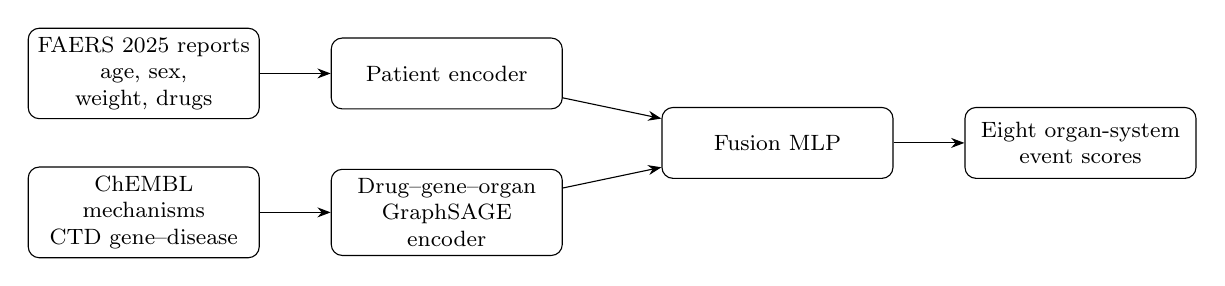
\begin{tikzpicture}[font=\footnotesize, node distance=6mm and 9mm, box/.style={draw, rounded corners, align=center, minimum height=9mm, text width=27mm}, >={Stealth}]
\node[box] (f) {FAERS 2025 reports\\age, sex, weight, drugs};
\node[box, below=of f] (c) {ChEMBL mechanisms\\CTD gene--disease};
\node[box, right=of f] (p) {Patient encoder};
\node[box, right=of c] (g) {Drug--gene--organ\\GraphSAGE encoder};
\node[box] (h) at ($(p)!0.5!(g)+(42mm,0)$) {Fusion MLP};
\node[box, right=of h] (o) {Eight organ-system\\event scores};
\draw[->] (f) -- (p);
\draw[->] (c) -- (g);
\draw[->] (p) -- (h);
\draw[->] (g) -- (h);
\draw[->] (h) -- (o);
\end{tikzpicture}
\caption{Overview of the pipeline. Patient attributes and mechanism knowledge are encoded separately, then combined to score organ systems for a report.}
\label{fig:pipe}
\end{figure*}

\textbf{Model.} Fig.~\ref{fig:pipe} summarizes the system. A two-layer heterogeneous GraphSAGE encoder~\cite{hamilton2017} produces a drug embedding $h_d$ from first-level ATC features and learned gene and organ embeddings. For each relation $r$, a layer aggregates neighbors and sums over relations:
\begin{equation}
h_v^{(l+1)} = \sigma\Big(\sum_{r} \mathrm{SAGE}_r\big(h_v^{(l)}, \{h_u^{(l)} : u \in \mathcal{N}_r(v)\}\big)\Big).
\end{equation}
A patient encoder maps the seven patient inputs $x$ to a 64-dimensional vector $z=f(x)$. A multilayer perceptron then gives organ probabilities,
\begin{equation}
\hat{y} = \mathrm{sigmoid}\big(g([h_d; z])\big) \in [0,1]^8,
\end{equation}
trained with binary cross-entropy over the eight organ labels. Because $h_d$ is computed from target neighbors and ATC features, the encoder can represent a drug with no training reports.

\textbf{Comparators.} We compare a global label rate, per-drug training frequency, patient features only, a learned drug-identity embedding with and without patient features, and the graph encoder with and without patient features.

\textbf{Evaluation.} The temporal split trains on the first three quarters and tests on the fourth. The cold-drug split holds out 20\% of drugs with graph targets, removing all of their reports from training while keeping their target edges. Identity models are excluded from this split because unseen drugs have untrained embeddings. Each setting uses five seeds, and the cold-drug split draws a new set of held-out drugs per seed. We report macro AUROC and AUPRC over organs. Within-drug AUROC is computed separately for drugs with at least 200 test reports and for organs with at least 20 positive and 20 negative reports in that drug, then averaged. Models without patient inputs score 0.5 by construction, so any gain reflects differences among patients on the same drug. Training used AdamW, early stopping on a 10\% validation sample and one RTX 5070 Ti Laptop GPU.

\section{Results}
\begin{table}[t]
\centering
\caption{Test performance, mean $\pm$ SD over five seeds.}
\label{tab:main}
\setlength{\tabcolsep}{3pt}
\begin{tabular}{llccc}
\toprule
Split & Model & AUROC & AUPRC & Within-drug \\
\midrule
Temporal & Global rate & .499 $\pm$ .001 & .181 $\pm$ .000 & .500 \\
 & Drug frequency & .711 $\pm$ .000 & .367 $\pm$ .000 & .500 \\
 & Patient only & .592 $\pm$ .001 & .258 $\pm$ .001 & .568 $\pm$ .000 \\
 & Drug ID & .711 $\pm$ .001 & .368 $\pm$ .001 & .500 \\
 & Drug ID + patient & \textbf{.732} $\pm$ .001 & \textbf{.397} $\pm$ .001 & \textbf{.588} $\pm$ .001 \\
 & Graph & .694 $\pm$ .001 & .345 $\pm$ .000 & .500 $\pm$ .001 \\
 & Graph + patient & .720 $\pm$ .001 & .381 $\pm$ .001 & .585 $\pm$ .002 \\
\midrule
Cold drug & Global rate & .501 $\pm$ .002 & .177 $\pm$ .002 & .500 \\
 & Patient only & .581 $\pm$ .007 & .247 $\pm$ .007 & .576 $\pm$ .006 \\
 & Graph & .604 $\pm$ .007 & .246 $\pm$ .006 & .500 \\
 & Graph + patient & \textbf{.639} $\pm$ .014 & \textbf{.284} $\pm$ .009 & \textbf{.582} $\pm$ .006 \\
\bottomrule
\end{tabular}
\end{table}

Table~\ref{tab:main} gives the main results. On the temporal split, adding patient features to drug identity improved AUROC over per-drug frequency by 0.020 (SD 0.001 across seeds). The graph model with patient features was 0.011 below the corresponding identity model, so mechanism structure gave no benefit when a drug already had report history.

On unseen drugs the pattern changed. Graph plus patient features exceeded patient features alone by 0.058 (SD 0.012) and exceeded the graph alone by 0.036 (SD 0.007). Both differences were positive in all five seeds. Five seeds support a consistent direction, not a formal significance claim.

Within-drug AUROC was 0.58--0.59 for models combining drug and patient inputs. The patient-only model already reached 0.568 on the temporal split, so most of this signal comes from the attributes themselves.

Table~\ref{tab:organ} shows that performance varies by organ. With report history, blood and liver events were easiest to rank and gastrointestinal events hardest. On unseen drugs, the graph gave its largest gains over patient features for kidney (+0.089), blood (+0.082) and nervous system events (+0.077), and its smallest for lung events (+0.021). A repeated full run changed mean graph-model AUROC by at most 0.001 and left every conclusion unchanged; reported values come from the final run.

\begin{table}[t]
\centering
\caption{Mean AUROC by organ system over five seeds.}
\label{tab:organ}
\begin{tabular}{lccc}
\toprule
 & Temporal & \multicolumn{2}{c}{Cold drug} \\
Organ & ID + patient & Patient only & Graph + patient \\
\midrule
Liver & .775 & .606 & .649 \\
Heart & .710 & .572 & .618 \\
Nervous & .696 & .558 & .634 \\
Kidney & .744 & .580 & .669 \\
Lung & .726 & .597 & .619 \\
Gastrointestinal & .685 & .570 & .616 \\
Skin & .712 & .574 & .636 \\
Blood & .805 & .592 & .674 \\
\bottomrule
\end{tabular}
\end{table}

\section{Discussion and Limitations}
The practical finding is conditional: report history is the stronger signal for established drugs, while mechanism knowledge helps when that history is absent. This is relevant to newly marketed drugs, although our held-out drugs are approved drugs with existing mechanism annotations.

These results describe patterns in reports, not risk. FAERS is voluntary, has no exposure denominator, and cannot establish causality. Reports are subject to under-reporting and stimulated reporting, and patient attributes may act as proxies for the indication. We condition on reports with at least one organ-mapped event, so outputs are not incidence estimates. Keyword labels are an approximation of standardized MedDRA grouping and were not reviewed by clinicians. Patient inputs omit laboratory values, comorbidities, dose and genotype, and weight is largely missing. Only the primary suspect drug is modeled, so drug--drug interactions are not addressed.

The current system is therefore a research prototype and must not guide treatment. Within-drug performance of 0.58--0.59 is far from what individual decisions would require.

\section{Conclusion}
We linked real adverse event reports to a mechanism graph and separated what each information source contributes. Patient attributes gave a small, consistent gain, and the graph improved prediction for drugs excluded from training. Future work should validate these findings on longitudinal clinical records with laboratory values, standardized MedDRA labels and clinician review.

\begin{thebibliography}{9}
\bibitem{zitnik2018} M. Zitnik, M. Agrawal, and J. Leskovec, ``Modeling polypharmacy side effects with graph convolutional networks,'' \emph{Bioinformatics}, vol. 34, no. 13, pp. i457--i466, 2018.
\bibitem{huang2024} K. Huang \emph{et al.}, ``A foundation model for clinician-centered drug repurposing,'' \emph{Nature Medicine}, 2024, doi: 10.1038/s41591-024-03233-x.
\bibitem{tatonetti2012} N. P. Tatonetti, P. P. Ye, R. Daneshjou, and R. B. Altman, ``Data-driven prediction of drug effects and interactions,'' \emph{Science Translational Medicine}, vol. 4, no. 125, 2012.
\bibitem{zdrazil2024} B. Zdrazil \emph{et al.}, ``The ChEMBL Database in 2023: a drug discovery platform spanning multiple bioactivity data types and time periods,'' \emph{Nucleic Acids Research}, vol. 52, no. D1, pp. D1180--D1192, 2024.
\bibitem{davis2023} A. P. Davis \emph{et al.}, ``Comparative Toxicogenomics Database (CTD): update 2023,'' \emph{Nucleic Acids Research}, vol. 51, no. D1, pp. D1257--D1262, 2023.
\bibitem{hamilton2017} W. Hamilton, Z. Ying, and J. Leskovec, ``Inductive representation learning on large graphs,'' in \emph{Advances in Neural Information Processing Systems}, 2017.
\end{thebibliography}

\end{document}
